\documentclass[]{article}

%opening
\title{Exercises Set 6}
\author{Paul Dubois}

\usepackage{amsmath}
\usepackage{amsfonts}
\usepackage{amsthm}
\usepackage{amssymb}
\usepackage{mathrsfs}
\usepackage{stmaryrd}
\usepackage{graphicx}

\newcommand{\Q}{\mathbb{Q}}
\newcommand{\N}{\mathbb{N}}
\newcommand{\Z}{\mathbb{Z}}
\newcommand{\R}{\mathbb{R}}
\newcommand{\Primes}{\mathbb{P}}
\newcommand{\st}{\text{ s.t. }}
\newcommand{\txtand}{\text{ and }}
\newcommand{\txtor}{\text{ or }}
\newcommand{\lxor}{\veebar}


\begin{document}
	
	\maketitle
	
	\begin{abstract}
		As this is the last session, there will be no compulsory questions this time.
	\end{abstract}	
	
	\section{Lagrangian multiplier technique}
	\begin{center}
		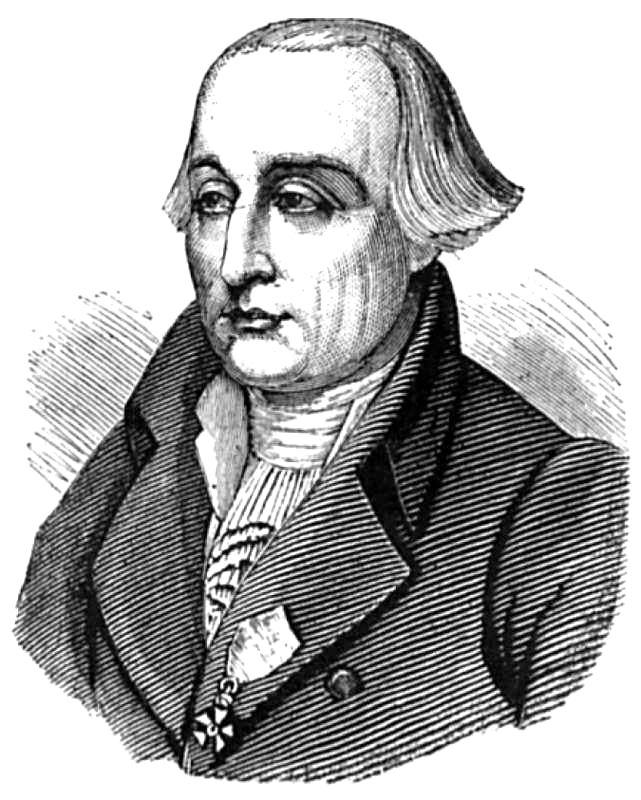
\includegraphics[height=4cm]{Lagrange}
	\end{center}

	\subsection{Unconstrained optimization}
	Let $f(x,y) = 2x^2-12x + 4y^2 + 8y + 20$.\\
	Find $(x^*,y^*) \in \R^2$ such that $f$ reaches its minimum (i.e. $f(x^*,y^*) \leq f(x,y) \quad \forall (x,y) \in \R^2$).
	
	\subsection{(Equality) Constrained optimization}
	Let $f(x,y) = 2x^2-12x + 4y^2 + 8y + 20$.\\
	Suppose further that we want $3x + 5y = 2$.\\
	Find $(x^*,y^*) \in \R^2$ such that $3x^* + 5y^* = 2$ and $f$ reaches its minimum (i.e. $f(x^*,y^*) \leq f(x,y) \quad \forall (x,y) \in \R^2,\ 3x + 5y = 2$).
	
	\subsection{Lagrange multiplier}
	Let $f(x,y) = 2x^2-12x + 4y^2 + 8y + 20$.\\
	Suppose further that we want $3x + 5y = 2$.\\
	Let $\mathcal{L}(x,y,\lambda) = f(x,y) - \lambda (3x + 5y -2)$.\\
	Find the point where $\nabla f = 0$
	
	\subsection{(Inequality) Constrained optimization}
	Let $f(x) = x^2-2x$.\\
	Suppose further that we want $3x \leq 2$.\\
	Find $x^* \in \R$ such that $3x^* \leq 2$ and $f$ reaches its minimum (i.e. $f(x^*) \leq f(x) \quad \forall x \in \R,\ 3x \leq 2$).
	\vspace{0.5cm}
	\\
	Let $f(x) = x^2+2x$.\\
	Suppose further that we want $3x \leq 2$.\\
	Find $x^* \in \R$ such that $3x^* \leq 2$ and $f$ reaches its minimum (i.e. $f(x^*) \leq f(x) \quad \forall x \in \R,\ 3x \leq 2$).
	
	
	\section{Support Vector Machines}
	\subsection{Theory}
	Define a line in $\R^2$ with parameters $\mathbf{w}$ and $b$ defined by $\mathbf{w}.\mathbf{x} = b$ (or $\mathbf{w}.\mathbf{x} - b = 0$) for $\mathbf{x} \in \R^2$.
	This line cut the plane in 2 regions:
	\begin{itemize}
		\item $\mathbf{x} \in \R^2$ such that $\mathbf{w}.\mathbf{x} - b < 0$
		\item $\mathbf{x} \in \R^2$ such that $\mathbf{w}.\mathbf{x} - b > 0$
	\end{itemize}
	The goal is to find $\mathbf{w}$ and $b$ such that all points of the first class are in the first region, and all points of the second class are in the second region.
	
	
	
	
	\subsection{Practice}
	The training dataset consists of the following data points:
	
	Positive class ("+1"):
	\begin{itemize}
		\item (2, 2)
		\item (1, 1)
	\end{itemize}
	
	Negative class ("-1"):
	\begin{itemize}
		\item (0, 1)
		\item (1, 0)
	\end{itemize}
	
	The SVM model's objective function for a linearly separable dataset is as follows:
	
	\[
	\text{Minimize } \frac{1}{2}\|\mathbf{w}\|^2
	\]
	
	Subject to the constraints:
	
	\[
	y_i(\mathbf{w}\cdot\mathbf{x}_i + b) \geq 1 \text{ for all } i
	\]
	
	Where:
	\begin{align*}
		y_i & \text{ is the class label } (+1 \text{ or } -1) \text{ of the } i\text{-th data point.} \\
		\mathbf{w} & \text{ is the weight vector of the hyperplane.} \\
		\mathbf{x}_i & \text{ is the } i\text{-th data point.} \\
		b & \text{ is the bias term.}
	\end{align*}
	
	Your tasks:
	\begin{enumerate}
		\item Calculate the optimal values of \(\mathbf{w}\) and \(b\) to separate the data points while maximizing the margin.
		
	\end{enumerate}
	
	1. Calculate the optimal values of \(\mathbf{w}\) and \(b\) to separate the data points while maximizing the margin.
	
	2. Determine the equation of the optimal hyperplane in the form \(\mathbf{w}\cdot\mathbf{x} + b = 0\).
	
	3. Identify the support vectors in the dataset.
	
	4. Calculate the margin, which is the perpendicular distance from the hyperplane to the nearest support vector.
	
	5. Classify a new data point, \((3, 2)\), based on the learned SVM model.
	
	Please provide the detailed steps and calculations for each task in your solution.
	
	
\end{document}
